\documentclass[aspectratio=169,10pt]{beamer}

\usetheme{Madrid}
\usecolortheme{default}

\definecolor{fptorange}{RGB}{221,132,82}
\definecolor{fptblue}{RGB}{76,114,176}
\definecolor{fptgreen}{RGB}{85,168,104}
\definecolor{fptred}{RGB}{196,78,82}

\setbeamercolor{palette primary}{bg=fptblue,fg=white}
\setbeamercolor{palette secondary}{bg=fptblue!80,fg=white}
\setbeamercolor{palette tertiary}{bg=fptblue!60,fg=white}
\setbeamercolor{structure}{fg=fptblue}
\setbeamercolor{block title}{bg=fptblue,fg=white}
\setbeamercolor{block body}{bg=fptblue!10}
\setbeamercolor{block title alerted}{bg=fptred,fg=white}
\setbeamercolor{block body alerted}{bg=fptred!10}
\setbeamercolor{block title example}{bg=fptgreen,fg=white}
\setbeamercolor{block body example}{bg=fptgreen!10}

\usepackage{graphicx}
\usepackage{booktabs}
\usepackage{amsmath}
\usepackage{hyperref}
\usepackage{tikz}
\usetikzlibrary{shapes.geometric, arrows.meta, positioning, fit}
\graphicspath{{figures/}}

\title[Agentic RAG for Curriculum Navigation]{Agentic RAG for University\\Curriculum Navigation}
\subtitle{Combining Semantic Retrieval with Structured Lookup Tools}
\author[Hoang et al.]{Anh~D.~D.~Hoang \and Khang~H.~Tran \and Nam~N.~Trinh}
\institute[FPT University]{Information Technology Specialization\\FPT University, Hanoi}
\date{DAP391m --- March 2026}

\begin{document}

% ------------------------------------------------------------------
% SLIDE 1: Title
% ------------------------------------------------------------------
\begin{frame}
\titlepage
\end{frame}


% ------------------------------------------------------------------
% SLIDE 2: Outline
% ------------------------------------------------------------------
\begin{frame}{Outline}
\tableofcontents
\end{frame}


% ==================================================================
\section{Problem \& Motivation}
% ==================================================================

% ------------------------------------------------------------------
% SLIDE 3: The Problem
% ------------------------------------------------------------------
\begin{frame}{The Problem}

\begin{columns}[T]
\begin{column}{0.55\textwidth}
Students need answers to questions like:
\begin{itemize}
    \item What are the prerequisites for Deep Learning?
    \item Can I accelerate to reach DPL302m by semester 4?
    \item Which specialization combo should I choose?
    \item I failed MAS291 --- what courses are blocked?
    \item How many tests does MAD101 have?
\end{itemize}

\vspace{0.5em}
\textbf{Current situation:}
\begin{itemize}
    \item Human advisors are overloaded
    \item Curriculum documents are scattered across files
    \item LLMs alone \textbf{hallucinate} course details
\end{itemize}
\end{column}

\begin{column}{0.4\textwidth}
\begin{alertblock}{LLM Hallucination Example}
\footnotesize
\textbf{Q:} How many credits is DPL302m?\\[0.3em]
\textbf{Baseline LLM:} ``DPL302m is typically a 3-credit course\ldots''\\[0.3em]
\textbf{Ground truth:} \textbf{6 credits}
\end{alertblock}
\end{column}
\end{columns}

\end{frame}


% ------------------------------------------------------------------
% SLIDE 4: Our Approach
% ------------------------------------------------------------------
\begin{frame}{Our Approach: Agentic RAG}

\begin{block}{Key Idea}
Combine \textbf{semantic vector search} (for open-ended content questions) with \textbf{deterministic structured tools} (for factual lookups), orchestrated by an \textbf{agentic loop} that calls multiple tools before answering.
\end{block}

\vspace{0.5em}

\begin{columns}[T]
\begin{column}{0.48\textwidth}
\textbf{Why not plain RAG?}
\begin{itemize}
    \item Prerequisite chains need recursive resolution
    \item Semester-course mappings are tabular
    \item Credit counts need exact lookup, not similarity
\end{itemize}
\end{column}
\begin{column}{0.48\textwidth}
\textbf{Why not Graph RAG?}
\begin{itemize}
    \item Only 9 source documents, 47 courses
    \item Relationships are explicitly listed in tables
    \item JSON lookup is deterministic and verifiable
\end{itemize}
\end{column}
\end{columns}

\end{frame}


% ==================================================================
\section{System Architecture}
% ==================================================================

% ------------------------------------------------------------------
% SLIDE 5: Data & Ingestion
% ------------------------------------------------------------------
\begin{frame}{Data Corpus \& Ingestion Pipeline}

\begin{columns}[T]
\begin{column}{0.45\textwidth}
\textbf{Raw data:} 9 markdown files
\begin{itemize}
    \item Syllabi (course content, assessments)
    \item Curriculum (47 courses, 10 semesters)
    \item Pathways (specialization combos)
\end{itemize}

\vspace{0.5em}
\textbf{Ingestion produces two outputs:}
\end{column}

\begin{column}{0.5\textwidth}
\footnotesize
\begin{exampleblock}{Vector Index}
\begin{itemize}
    \item MarkdownHeaderTextSplitter (H2 sections)
    \item RecursiveCharacterTextSplitter (500 chars)
    \item Min chunk filter: 50 chars
    \item 8,446 $\rightarrow$ \textbf{6,256 chunks}
    \item OpenAI text-embedding-3-small (1536-d)
    \item Pinecone Serverless (cosine)
\end{itemize}
\end{exampleblock}

\begin{exampleblock}{Structured Tables}
\begin{itemize}
    \item course\_index (47 courses)
    \item prerequisites (23 entries)
    \item curriculum\_map (10 semesters)
    \item combo\_map (5 pathways)
    \item programme\_outcomes, PLOs
\end{itemize}
\end{exampleblock}
\end{column}
\end{columns}

\end{frame}


% ------------------------------------------------------------------
% SLIDE 6: Agent Graph (Architecture Diagram)
% ------------------------------------------------------------------
\begin{frame}{Agent Graph Architecture}

\centering
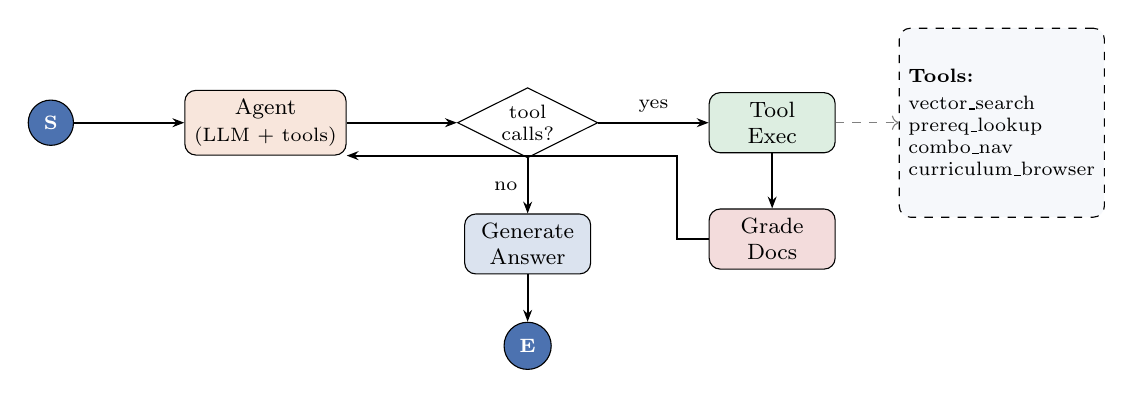
\begin{tikzpicture}[
    node distance=0.8cm and 1.4cm,
    every node/.style={font=\footnotesize},
    process/.style={rectangle, rounded corners, draw, minimum width=1.6cm, minimum height=0.6cm, align=center},
    decision/.style={diamond, draw, aspect=2, inner sep=1pt, align=center, font=\scriptsize},
    startstop/.style={circle, draw, fill=fptblue, text=white, minimum size=0.5cm, font=\scriptsize\bfseries},
    arrow/.style={-{Stealth[length=1.5mm]}, thick},
]

\node[startstop] (start) {S};
\node[process, fill=fptorange!20, right=of start] (agent) {Agent\\{\scriptsize(LLM + tools)}};
\node[decision, right=of agent] (hastools) {tool\\calls?};
\node[process, fill=fptgreen!20, right=of hastools] (tools) {Tool\\Exec};
\node[process, fill=fptred!20, below=0.7cm of tools] (grade) {Grade\\Docs};
\node[process, fill=fptblue!20, below=0.7cm of hastools] (generate) {Generate\\Answer};
\node[startstop, below=0.6cm of generate] (end) {E};

\draw[arrow] (start) -- (agent);
\draw[arrow] (agent) -- (hastools);
\draw[arrow] (hastools) -- node[above, font=\scriptsize] {yes} (tools);
\draw[arrow] (hastools) -- node[left, font=\scriptsize] {no} (generate);
\draw[arrow] (tools) -- (grade);
\draw[arrow] (grade.west) -- +(-0.4,0) |- (agent.south east);
\draw[arrow] (generate) -- (end);

\node[draw, dashed, rounded corners, fill=fptblue!5,
      right=0.8cm of tools, minimum width=2.2cm, minimum height=2.4cm, align=left, font=\scriptsize] (toolbox) {
    \textbf{Tools:}\\[0.2em]
    vector\_search\\
    prereq\_lookup\\
    combo\_nav\\
    curriculum\_browser
};

\draw[dashed, ->, gray] (tools.east) -- (toolbox.west);

\end{tikzpicture}

\vspace{0.3em}
\footnotesize
Agent loops up to \textbf{6 tool calls}. Structured tools skip grading. Only \texttt{vector\_search} is graded (1 rewrite attempt).

\end{frame}


% ------------------------------------------------------------------
% SLIDE 7: The Four Tools
% ------------------------------------------------------------------
\begin{frame}{Tool Definitions}

\begin{columns}[T]
\begin{column}{0.48\textwidth}

\begin{block}{\texttt{vector\_search}(q, code, type)}
Semantic search over Pinecone\\
\footnotesize
\textit{Use for:} course content, learning outcomes, assessments, session topics, materials
\end{block}

\vspace{0.3em}

\begin{block}{\texttt{prerequisite\_lookup}(code, dir)}
Recursive prerequisite chain resolver\\
\footnotesize
\textit{Forward:} what do I need before X?\\
\textit{Reverse:} what does X unlock?
\end{block}

\end{column}
\begin{column}{0.48\textwidth}

\begin{block}{\texttt{combo\_navigator}(id, topic)}
Browse specialization pathways\\
\footnotesize
\textit{Use for:} which combos exist, what courses in a combo, elective options
\end{block}

\vspace{0.3em}

\begin{block}{\texttt{curriculum\_browser}(sem, code)}
Semester-level curriculum data\\
\footnotesize
\textit{Use for:} courses in semester X, credit counts, full study plan overview
\end{block}

\end{column}
\end{columns}

\vspace{0.5em}
All tools include \textbf{fuzzy course code resolution}: ``AIL'' $\rightarrow$ ``AIL303m''

\end{frame}


% ------------------------------------------------------------------
% SLIDE 8: Student Personalization
% ------------------------------------------------------------------
\begin{frame}{Student Personalization}

\begin{columns}[T]
\begin{column}{0.45\textwidth}
\textbf{Student profiles contain:}
\begin{itemize}
    \item Current semester
    \item Passed courses with grades
    \item Failed courses (must retake)
    \item Computed GPA
\end{itemize}

\vspace{0.5em}
\textbf{FPT academic rules encoded:}
\begin{itemize}
    \item 10-week semesters, 1-month breaks
    \item Max 2 extra courses/semester
    \item Retake allowed for GPA improvement
\end{itemize}
\end{column}

\begin{column}{0.5\textwidth}
\begin{exampleblock}{Example: Struggling Student}
\footnotesize
\textbf{Pham Duc Huy} --- Semester 4\\
\textbf{Failed:} MAS291 (3.5/10)\\
\textbf{Low grades:} MAE101 (5.0), MAD101 (4.5)\\[0.5em]
\textbf{Q:} Do I have to retake any course?\\[0.3em]
\textbf{Agent:} ``You must retake \textbf{MAS291}. This blocks \textbf{AIL303m} (Machine Learning) and transitively \textbf{DPL302m} (Deep Learning). You can take AI17\_COM*1, AI17\_COM*2, and DWP301c in Semester 5.''
\end{exampleblock}
\end{column}
\end{columns}

\end{frame}


% ==================================================================
\section{Evaluation}
% ==================================================================

% ------------------------------------------------------------------
% SLIDE 9: Experimental Setup
% ------------------------------------------------------------------
\begin{frame}{Experimental Setup}

\begin{columns}[T]
\begin{column}{0.48\textwidth}
\begin{block}{Golden Test Set}
\textbf{48 questions} across 5 categories:
\footnotesize
\begin{tabular}{lr}
\toprule
Category & Count \\
\midrule
Factual Lookup & 10 \\
Prerequisite Reasoning & 10 \\
Combo Pathway & 8 \\
Cross Document & 10 \\
Curriculum Planning & 10 \\
\bottomrule
\end{tabular}
\normalsize
\vspace{0.3em}\\
Each with reference answer and expected tool.
\end{block}
\end{column}

\begin{column}{0.48\textwidth}
\begin{block}{Evaluation Metrics (LLM-as-Judge)}
GPT-4o-mini scores on $[0, 1]$:
\begin{itemize}
    \item \textbf{Relevancy}: addresses the question?
    \item \textbf{Faithfulness}: grounded in context?
    \item \textbf{Correctness}: matches reference?
\end{itemize}
\end{block}

\vspace{0.3em}
\begin{block}{Systems Compared}
\begin{itemize}
    \item \textbf{RAG}: Full agent + 4 tools
    \item \textbf{Baseline}: GPT-4o-mini only
\end{itemize}
Both at temperature = 0.
\end{block}
\end{column}
\end{columns}

\end{frame}


% ------------------------------------------------------------------
% SLIDE 10: Overall Results
% ------------------------------------------------------------------
\begin{frame}{Overall Results}

\begin{columns}[T]
\begin{column}{0.45\textwidth}

\begin{table}
\footnotesize
\centering
\begin{tabular}{lccc}
\toprule
\textbf{Metric} & \textbf{RAG} & \textbf{Base} & \textbf{$\Delta$} \\
\midrule
Relevancy & 0.958 & 0.948 & +0.010 \\
Faithfulness & \textbf{0.865} & 0.000 & \textbf{+0.865} \\
Correctness & \textbf{0.625} & 0.240 & \textbf{+0.385} \\
\bottomrule
\end{tabular}
\end{table}

\vspace{0.5em}
Key findings:
\begin{itemize}
    \item \textbf{+160.4\%} relative correctness improvement
    \item Faithfulness: 0 $\rightarrow$ 0.865
    \item Relevancy comparable (both $\sim$0.95)
\end{itemize}

\end{column}
\begin{column}{0.52\textwidth}
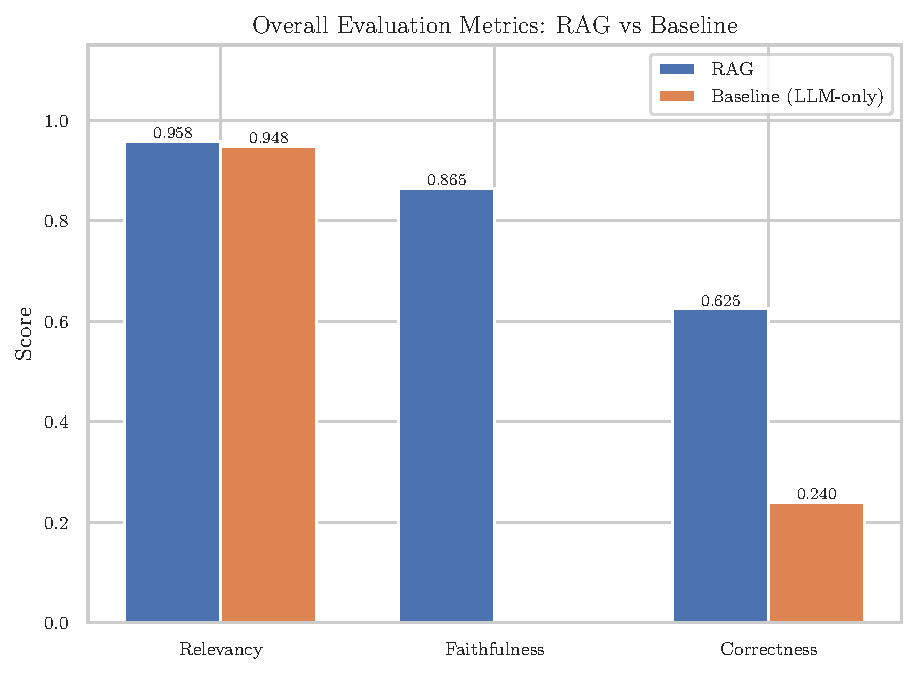
\includegraphics[width=\textwidth]{overall_comparison.pdf}
\end{column}
\end{columns}

\end{frame}


% ------------------------------------------------------------------
% SLIDE 11: Per-Category Results
% ------------------------------------------------------------------
\begin{frame}{Per-Category Correctness}

\begin{columns}[T]
\begin{column}{0.42\textwidth}

\footnotesize
\begin{tabular}{lccc}
\toprule
\textbf{Category} & \textbf{RAG} & \textbf{Base} & \textbf{$\Delta$} \\
\midrule
Factual & 0.700 & 0.150 & \textcolor{fptgreen}{+0.550} \\
Combo & 0.688 & 0.188 & \textcolor{fptgreen}{+0.500} \\
Prereq & 0.600 & 0.150 & \textcolor{fptgreen}{+0.450} \\
Planning & 0.600 & 0.250 & \textcolor{fptgreen}{+0.350} \\
Cross-doc & 0.550 & 0.450 & +0.100 \\
\bottomrule
\end{tabular}

\normalsize
\vspace{0.7em}
\textbf{Largest gains:}
\begin{itemize}
    \item Factual lookup: \textbf{+0.550}
    \item Combo pathways: \textbf{+0.500}
\end{itemize}

\textbf{Smallest gain:}
\begin{itemize}
    \item Cross-document: +0.100
\end{itemize}

\end{column}
\begin{column}{0.55\textwidth}
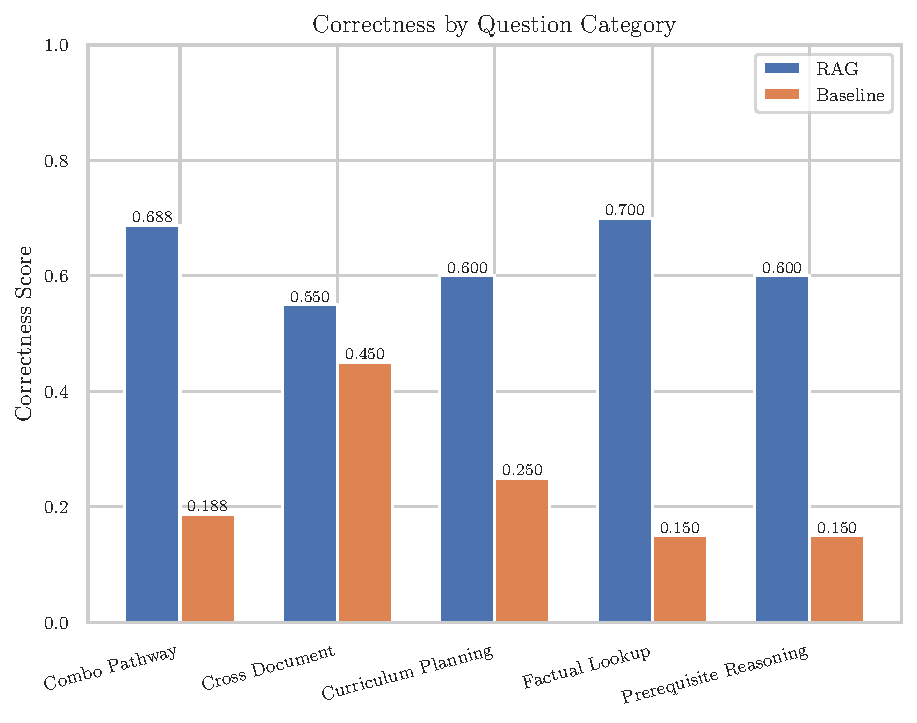
\includegraphics[width=\textwidth]{category_correctness.pdf}
\end{column}
\end{columns}

\end{frame}


% ------------------------------------------------------------------
% SLIDE 12: Score Distribution
% ------------------------------------------------------------------
\begin{frame}{Score Distribution}

\begin{center}
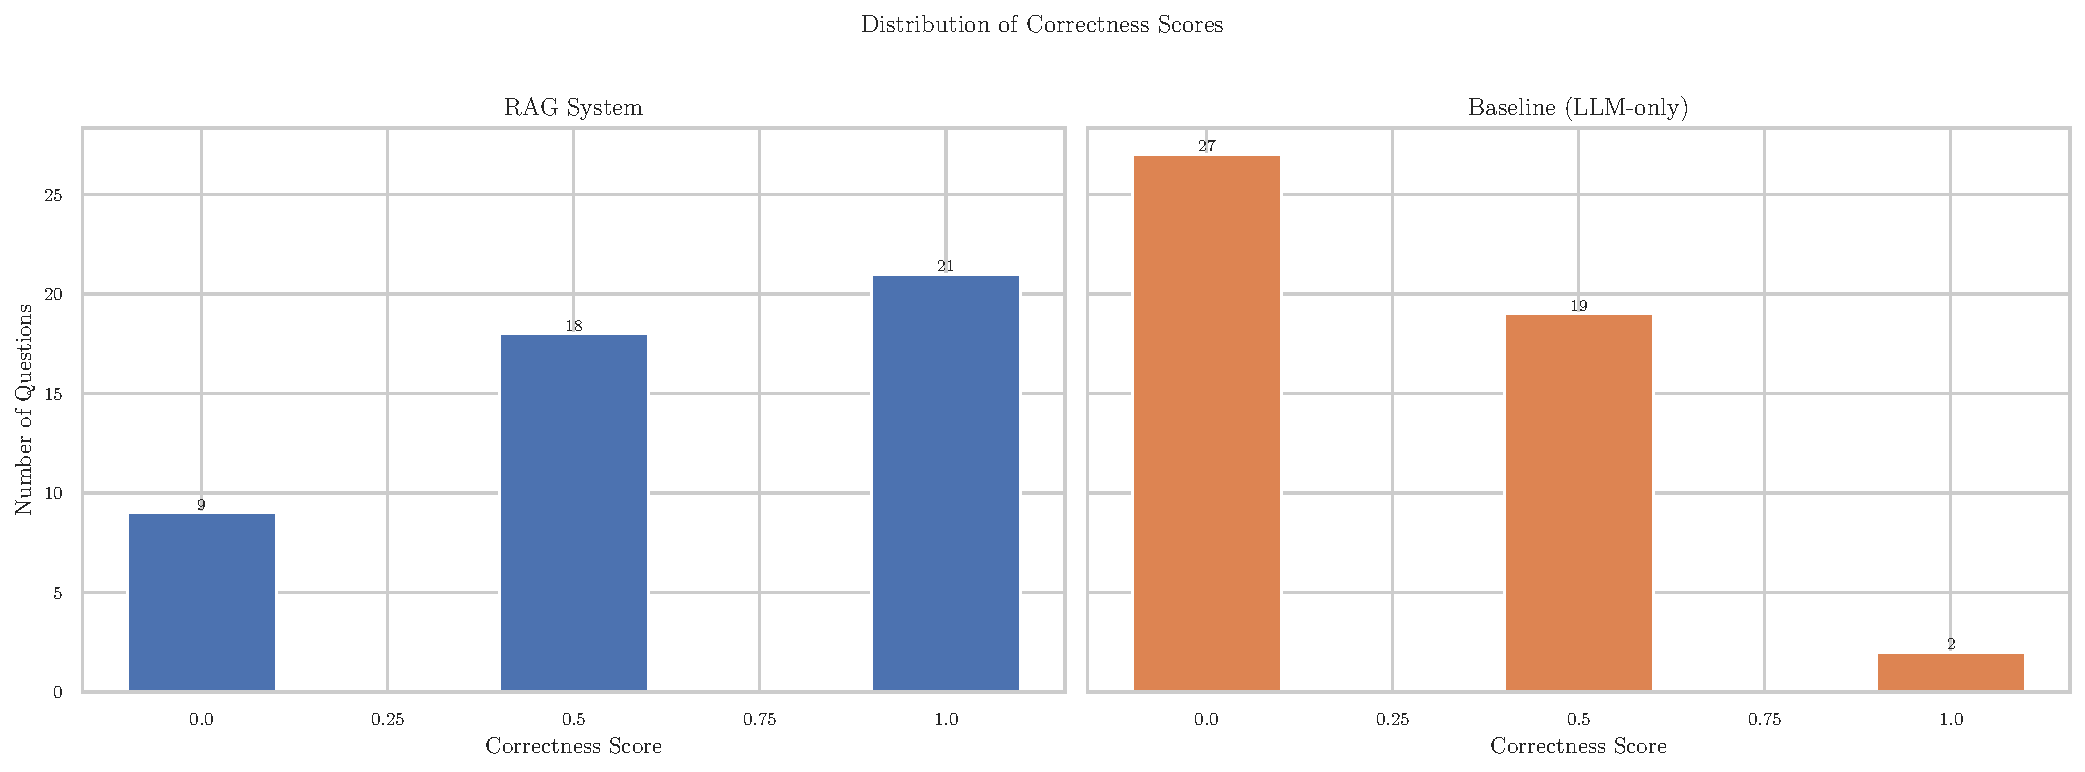
\includegraphics[width=0.85\textwidth]{score_distribution.pdf}
\end{center}

\vspace{-0.5em}
\footnotesize
RAG produces \textbf{19 fully correct} answers (1.0) vs.\ \textbf{5} for baseline.\\
RAG has \textbf{9 failures} (0.0) vs.\ \textbf{27} for baseline.

\end{frame}


% ------------------------------------------------------------------
% SLIDE 13: Tool Usage
% ------------------------------------------------------------------
\begin{frame}{Tool Usage Patterns}

\begin{columns}[T]
\begin{column}{0.48\textwidth}
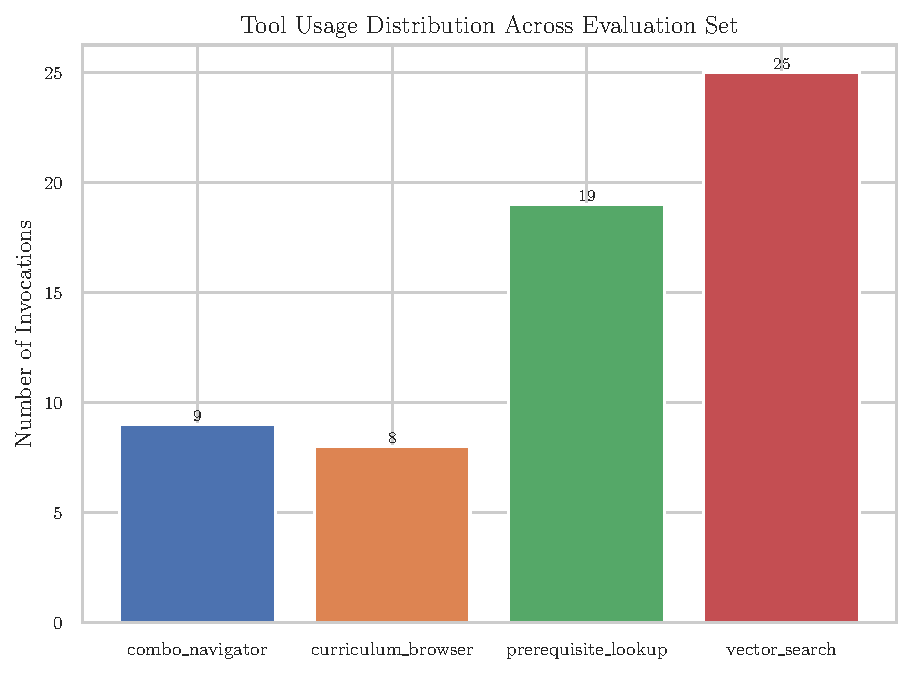
\includegraphics[width=\textwidth]{tool_usage.pdf}
\end{column}
\begin{column}{0.48\textwidth}

\vspace{1em}
\textbf{Observations:}
\begin{itemize}
    \item \texttt{vector\_search} most frequent --- content questions dominate
    \item \texttt{prerequisite\_lookup} for dependency chains
    \item \texttt{curriculum\_browser} for semester/credit queries
    \item \texttt{combo\_navigator} for specialization questions
\end{itemize}

\vspace{0.5em}
\textbf{Multi-tool queries:}\\
Complex questions invoke 2--3 tools in sequence.\\
Example: ``Can I accelerate to DPL302m?''\\
$\rightarrow$ \texttt{prerequisite\_lookup} + \texttt{curriculum\_browser}

\end{column}
\end{columns}

\end{frame}


% ------------------------------------------------------------------
% SLIDE 14: Faithfulness Impact
% ------------------------------------------------------------------
\begin{frame}{Why Faithfulness Matters}

\begin{columns}[T]
\begin{column}{0.48\textwidth}
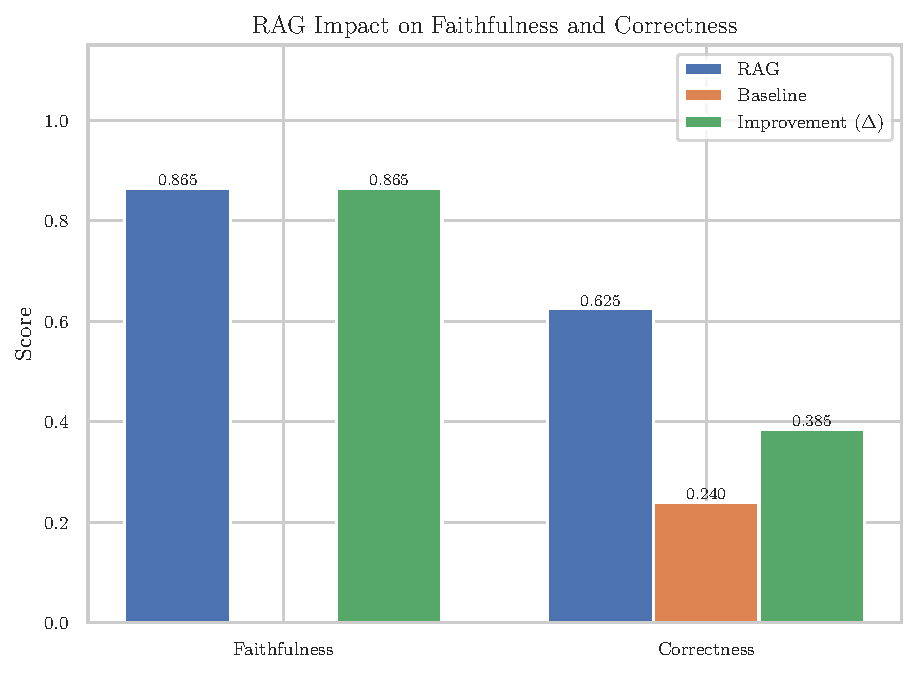
\includegraphics[width=\textwidth]{faithfulness_impact.pdf}
\end{column}
\begin{column}{0.48\textwidth}

\vspace{1em}
\textbf{Baseline (no tools):}
\begin{itemize}
    \item Faithfulness = \textbf{0.000}
    \item No context $\rightarrow$ no grounding
    \item Invents course codes, credits, semesters
\end{itemize}

\vspace{0.5em}
\textbf{RAG (with tools):}
\begin{itemize}
    \item Faithfulness = \textbf{0.865}
    \item Answers cite actual tool results
    \item Verifiable against source data
\end{itemize}

\vspace{0.5em}
\begin{alertblock}{Takeaway}
\footnotesize
Tool access is \textit{necessary} for trustworthy curriculum advising. LLMs alone cannot be trusted with factual academic data.
\end{alertblock}

\end{column}
\end{columns}

\end{frame}


% ==================================================================
\section{Discussion \& Lessons Learned}
% ==================================================================

% ------------------------------------------------------------------
% SLIDE 15: Failure Analysis
% ------------------------------------------------------------------
\begin{frame}{Failure Analysis}

\begin{columns}[T]
\begin{column}{0.48\textwidth}

\textbf{RAG failures} (9/48 = 18.8\%):

\begin{enumerate}
    \item \textbf{Credit confusion} (fact\_01, 04, 09)\\
    \footnotesize vector\_search retrieves chunks without credit data; curriculum\_browser not called as fallback\normalsize

    \item \textbf{Incomplete prereq chains} (prereq\_03, 06)\\
    \footnotesize Deep 3+ level hierarchies partially resolved\normalsize

    \item \textbf{Cross-doc synthesis} (content\_03, 09)\\
    \footnotesize Multi-source queries need multiple vector searches; coverage gaps\normalsize
\end{enumerate}

\end{column}
\begin{column}{0.48\textwidth}

\textbf{Baseline failures} (27/48 = 56.3\%):

\begin{alertblock}{Systematic Errors}
\footnotesize
\begin{itemize}
    \item Invents nonexistent course codes
    \item Wrong semester numbers (sem 6 instead of 4)
    \item Inaccurate totals (40 subjects vs.\ actual 47)
    \item Fabricates prerequisite relationships
\end{itemize}
\end{alertblock}

\vspace{0.3em}
\textbf{Key difference:}\\
RAG failures are \textit{incomplete} answers.\\
Baseline failures are \textit{incorrect} answers.

\end{column}
\end{columns}

\end{frame}


% ------------------------------------------------------------------
% SLIDE 16: Key Design Decisions
% ------------------------------------------------------------------
\begin{frame}{Key Design Decisions}

\begin{enumerate}
    \item \textbf{Structured tools over Graph RAG}
    \begin{itemize}
        \footnotesize
        \item 9 documents, 47 courses --- too small for knowledge graph overhead
        \item All relationships explicitly listed $\rightarrow$ JSON lookup is deterministic
        \item Result: structured tools achieve higher correctness than vector search
    \end{itemize}

    \vspace{0.3em}
    \item \textbf{Multi-tool loop instead of single-pass}
    \begin{itemize}
        \footnotesize
        \item Original design: agent $\rightarrow$ tool $\rightarrow$ generate (one tool only)
        \item Problem: ``Can I accelerate to DPL302m?'' needs 2+ tools
        \item Fix: agent $\leftrightarrow$ tools loop with safety counter (max 6)
    \end{itemize}

    \vspace{0.3em}
    \item \textbf{Current-turn-only generation}
    \begin{itemize}
        \footnotesize
        \item Problem: generate node saw full conversation history, repeated old answers
        \item Fix: extract only current question + its tool results for synthesis
    \end{itemize}

    \vspace{0.3em}
    \item \textbf{Selective grading}
    \begin{itemize}
        \footnotesize
        \item Only \texttt{vector\_search} graded --- structured tools are always relevant
        \item Query rewriting preserves course code prefixes (avoids ``MAE'' $\rightarrow$ ``Master of Arts'')
    \end{itemize}
\end{enumerate}

\end{frame}


% ==================================================================
\section{Demo \& Future Work}
% ==================================================================

% ------------------------------------------------------------------
% SLIDE 17: Demo
% ------------------------------------------------------------------
\begin{frame}{Live Demo}

\begin{center}
\Large
\textit{Streamlit UI Demo}

\vspace{1em}
\normalsize

\begin{tabular}{ll}
\toprule
\textbf{Feature} & \textbf{Description} \\
\midrule
Profile selector & 5 predefined student personas \\
Chat interface & Multi-turn conversation \\
Source citations & Expandable tool call results \\
Profile details & Passed/failed courses, GPA \\
\bottomrule
\end{tabular}

\vspace{1em}
\texttt{\$ streamlit run src/app.py}
\end{center}

\end{frame}


% ------------------------------------------------------------------
% SLIDE 18: Technology Stack
% ------------------------------------------------------------------
\begin{frame}{Technology Stack}

\begin{center}
\footnotesize
\begin{tabular}{lll}
\toprule
\textbf{Layer} & \textbf{Technology} & \textbf{Details} \\
\midrule
LLM & GPT-4o-mini & temperature=0, via LangChain \\
Embeddings & text-embedding-3-small & 1,536 dimensions \\
Vector DB & Pinecone Serverless & AWS us-east-1, cosine \\
Agent & LangGraph & StateGraph with conditional edges \\
UI & Streamlit & Chat interface with sidebar \\
Config & Pydantic-Settings & .env-based configuration \\
Logging & Loguru & Structured logging \\
Package mgmt & uv & Fast Python package manager \\
\bottomrule
\end{tabular}
\end{center}

\end{frame}


% ------------------------------------------------------------------
% SLIDE 19: Future Work
% ------------------------------------------------------------------
\begin{frame}{Limitations \& Future Work}

\textbf{Current limitations:}
\begin{itemize}
    \item LLM-as-judge evaluation (no human judges yet)
    \item 48-question test set is relatively small
    \item Only K20-K21 curriculum version
    \item Cross-document synthesis remains weak (+0.100)
\end{itemize}

\vspace{0.7em}
\textbf{Future directions:}
\begin{itemize}
    \item Human evaluation study with real students
    \item Multi-curriculum version support (K18-K19, K22+)
    \item Multi-hop retrieval for cross-document questions
    \item Real deployment with user feedback collection
    \item Fine-tuned embedding model on curriculum domain
\end{itemize}

\end{frame}


% ------------------------------------------------------------------
% SLIDE 20: Summary
% ------------------------------------------------------------------
\begin{frame}{Summary}

\begin{block}{What We Built}
An agentic RAG chatbot for curriculum advising that combines semantic vector search with deterministic structured tools, orchestrated by a LangGraph state machine.
\end{block}

\vspace{0.3em}

\begin{columns}[T]
\begin{column}{0.48\textwidth}
\begin{exampleblock}{Key Results}
\begin{itemize}
    \item Correctness: 0.625 vs.\ 0.240 \textbf{(+160\%)}
    \item Faithfulness: 0.865 vs.\ 0.000
    \item 19/48 fully correct vs.\ 5/48
\end{itemize}
\end{exampleblock}
\end{column}
\begin{column}{0.48\textwidth}
\begin{exampleblock}{Key Contributions}
\begin{itemize}
    \item Hybrid retrieval architecture
    \item Multi-tool agentic loop
    \item Empirical RAG vs.\ baseline comparison
\end{itemize}
\end{exampleblock}
\end{column}
\end{columns}

\vspace{0.5em}
\begin{center}
\Large Thank you! Questions?
\end{center}

\end{frame}


\end{document}
